\section{Clustering: K-Means}
% \begin{frame}{What is Clustering?}

% \textbf{Goal:} Group similar data points together without labels

% \vspace{0.5em}
% \begin{columns}[c]
% \begin{column}{0.48\textwidth}
% \textbf{Supervised vs Unsupervised}

% \vspace{0.5em}
% \begin{tcolorbox}[colback=blue!5, colframe=blue!50]
% \textbf{Supervised}\\
% \small
% Data: $(x, y)$ with labels\\
% Goal: Learn $f(x) \rightarrow y$\\
% Example: Cat vs Dog classifier
% \end{tcolorbox}

% \vspace{0.3em}
% \begin{tcolorbox}[colback=green!5, colframe=green!50!black]
% \textbf{Unsupervised (Clustering)}\\
% \small
% Data: $x$ only, no labels\\
% Goal: Find natural groups\\
% Example: Customer segments
% \end{tcolorbox}
% \end{column}

% \begin{column}{0.48\textwidth}
% \centering
% \textbf{Example: Customer Data}

% \begin{tikzpicture}[scale=0.8]
%     \begin{axis}[
%         width=5.5cm, height=5cm,
%         xlabel={Age},
%         ylabel={Income},
%         grid=major,
%         xmin=20, xmax=70,
%         ymin=20, ymax=90
%     ]
    
%     % Young, low income (students)
%     \addplot[only marks, mark=*, mark size=2pt, blue!70] coordinates {
%         (25,25) (28,30) (22,28) (26,32) (24,27)
%         (27,29) (23,26) (29,31) (26,28)
%     };
    
%     % Middle age, medium income (professionals)
%     \addplot[only marks, mark=*, mark size=2pt, red!70] coordinates {
%         (40,55) (42,58) (38,52) (43,60) (41,56)
%         (39,54) (44,59) (40,57) (42,55)
%     };
    
%     % Older, high income (executives)
%     \addplot[only marks, mark=*, mark size=2pt, green!60!black] coordinates {
%         (55,75) (58,78) (52,72) (60,80) (56,76)
%         (54,74) (59,79) (57,77) (55,75)
%     };
    
%     \end{axis}
% \end{tikzpicture}

% \vspace{0.3em}
% \small Can we find groups automatically?
% \end{column}
% \end{columns}

% \vspace{0.5em}
% \centering
% \textbf{K-Means is one of the most popular clustering algorithms!}

% \end{frame}

\section{Clustering: K-Means}

% --- SLIDE 2: K-Means Intuition ---
\begin{frame}{Clustering: K-Means}

\textbf{Main Idea:} Represent each cluster by its center (mean)

\vspace{0.5em}
\centering
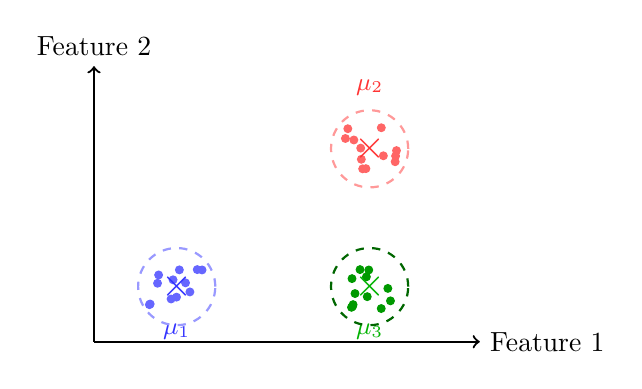
\begin{tikzpicture}[scale=0.7]
    % Cluster 1 (bottom-left) - Blue
    \foreach \i in {1,...,12} {
        \pgfmathsetmacro{\x}{1.5 + 0.5*rand}
        \pgfmathsetmacro{\y}{1 + 0.4*rand}
        \filldraw[blue!60] (\x, \y) circle (2pt);
    }
    \node[blue!80, font=\Large] at (1.5, 1) {$\times$};
    \node[blue!80, font=\small, below] at (1.5, 0.5) {$\mu_1$};
    \draw[blue!40, thick, dashed] (1.5, 1) circle (0.7cm);
    
    % Cluster 2 (top-right) - Red
    \foreach \i in {1,...,12} {
        \pgfmathsetmacro{\x}{5 + 0.5*rand}
        \pgfmathsetmacro{\y}{3.5 + 0.4*rand}
        \filldraw[red!60] (\x, \y) circle (2pt);
    }
    \node[red!80, font=\Large] at (5, 3.5) {$\times$};
    \node[red!80, font=\small, above] at (5, 4.3) {$\mu_2$};
    \draw[red!40, thick, dashed] (5, 3.5) circle (0.7cm);
    
    % Cluster 3 (bottom-right) - Green
    \foreach \i in {1,...,12} {
        \pgfmathsetmacro{\x}{5 + 0.5*rand}
        \pgfmathsetmacro{\y}{1 + 0.4*rand}
        \filldraw[green!60!black] (\x, \y) circle (2pt);
    }
    \node[green!70!black, font=\Large] at (5, 1) {$\times$};
    \node[green!70!black, font=\small, below] at (5, 0.5) {$\mu_3$};
    \draw[green!40!black, thick, dashed] (5, 1) circle (0.7cm);
    
    % Axes
    \draw[->, thick] (0, 0) -- (7, 0) node[right] {Feature 1};
    \draw[->, thick] (0, 0) -- (0, 5) node[above] {Feature 2};
\end{tikzpicture}

\vspace{0.8em}
\begin{itemize}
\item Each cluster has a \textbf{center} (centroid) $\mu_k$ (marked with $\times$)
\item Points belong to their \textbf{nearest} center
\item Goal: Find centers that minimize total distance to assigned points
\end{itemize}

\end{frame}

% --- SLIDE 3: K-Means Algorithm ---
\begin{frame}[allowframebreaks]{K-Means Algorithm}

\begin{tcolorbox}[colback=blue!5, colframe=blue!50, title=\textbf{K-Means Algorithm}]

\textbf{Input:} Data $\{x_1, x_2, \ldots, x_n\}$ and number of clusters $K$

\vspace{0.5em}
\textbf{Initialize:} Randomly place $K$ cluster centers $\mu_1, \mu_2, \ldots, \mu_K$

\vspace{0.5em}
\textbf{Repeat until convergence:}

\vspace{0.3em}
\begin{enumerate}
\item \textbf{Assignment Step:} For each point $x_i$, assign to nearest center
\[
c_i = \arg\min_{k=1,\ldots,K} \|x_i - \mu_k\|^2
\]
\small (find which center is closest)

\vspace{0.5em}
\item \textbf{Update Step:} Move each center to mean of assigned points
\[
\mu_k = \frac{1}{|C_k|} \sum_{i \in C_k} x_i
\]
\small (average all points in cluster $k$)
\end{enumerate}

\vspace{0.5em}
\textbf{Stop when:} Assignments don't change OR max iterations reached
\end{tcolorbox}

\end{frame}

% --- SLIDE 4: K-Means Step-by-Step Visualization ---
\begin{frame}{K-Means: Step-by-Step Example}

\centering
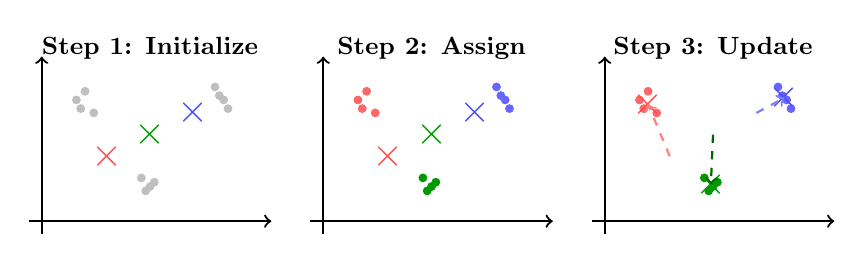
\begin{tikzpicture}[scale=0.55]
    % Step 1: Initial random centers
    \begin{scope}[shift={(0,0)}]
        \node[font=\small\bfseries] at (2.5, 4) {Step 1: Initialize};
        \draw[->, thick] (-0.3, 0) -- (5.3, 0);
        \draw[->, thick] (0, -0.3) -- (0, 3.8);
        
        % Data points (all gray initially)
        \foreach \x/\y in {0.8/2.8, 1.2/2.5, 1.0/3.0, 0.9/2.6,
                           4.2/2.8, 4.0/3.1, 4.3/2.6, 4.1/2.9,
                           2.5/0.8, 2.3/1.0, 2.6/0.9, 2.4/0.7} {
            \filldraw[gray!50] (\x, \y) circle (2.5pt);
        }
        
        % Random initial centers
        \node[red!70, font=\Large] at (1.5, 1.5) {$\times$};
        \node[blue!70, font=\Large] at (3.5, 2.5) {$\times$};
        \node[green!60!black, font=\Large] at (2.5, 2.0) {$\times$};
    \end{scope}
    
    % Step 2: Assign to nearest
    \begin{scope}[shift={(6.5,0)}]
        \node[font=\small\bfseries] at (2.5, 4) {Step 2: Assign};
        \draw[->, thick] (-0.3, 0) -- (5.3, 0);
        \draw[->, thick] (0, -0.3) -- (0, 3.8);
        
        % Points colored by assignment
        \foreach \x/\y in {0.8/2.8, 1.2/2.5, 1.0/3.0, 0.9/2.6} {
            \filldraw[red!60] (\x, \y) circle (2.5pt);
        }
        \foreach \x/\y in {4.2/2.8, 4.0/3.1, 4.3/2.6, 4.1/2.9} {
            \filldraw[blue!60] (\x, \y) circle (2.5pt);
        }
        \foreach \x/\y in {2.5/0.8, 2.3/1.0, 2.6/0.9, 2.4/0.7} {
            \filldraw[green!60!black] (\x, \y) circle (2.5pt);
        }
        
        % Old centers
        \node[red!70, font=\Large] at (1.5, 1.5) {$\times$};
        \node[blue!70, font=\Large] at (3.5, 2.5) {$\times$};
        \node[green!60!black, font=\Large] at (2.5, 2.0) {$\times$};
    \end{scope}
    
    % Step 3: Update centers
    \begin{scope}[shift={(13,0)}]
        \node[font=\small\bfseries] at (2.5, 4) {Step 3: Update};
        \draw[->, thick] (-0.3, 0) -- (5.3, 0);
        \draw[->, thick] (0, -0.3) -- (0, 3.8);
        
        % Points (same as step 2)
        \foreach \x/\y in {0.8/2.8, 1.2/2.5, 1.0/3.0, 0.9/2.6} {
            \filldraw[red!60] (\x, \y) circle (2.5pt);
        }
        \foreach \x/\y in {4.2/2.8, 4.0/3.1, 4.3/2.6, 4.1/2.9} {
            \filldraw[blue!60] (\x, \y) circle (2.5pt);
        }
        \foreach \x/\y in {2.5/0.8, 2.3/1.0, 2.6/0.9, 2.4/0.7} {
            \filldraw[green!60!black] (\x, \y) circle (2.5pt);
        }
        
        % NEW centers (moved to cluster means)
        \node[red!70, font=\Large] at (1.0, 2.7) {$\times$};
        \node[blue!70, font=\Large] at (4.15, 2.85) {$\times$};
        \node[green!60!black, font=\Large] at (2.45, 0.85) {$\times$};
        
        % Arrows showing movement
        \draw[->, red!50, thick, dashed] (1.5, 1.5) -- (1.0, 2.7);
        \draw[->, blue!50, thick, dashed] (3.5, 2.5) -- (4.15, 2.85);
        \draw[->, green!40!black, thick, dashed] (2.5, 2.0) -- (2.45, 0.85);
    \end{scope}
\end{tikzpicture}

\vspace{0.8em}
\textbf{Repeat steps 2-3} until centers stop moving (typically 10-100 iterations)

\end{frame}

% --- SLIDE 5: Choosing K (Elbow Method) ---
\begin{frame}{How to Choose K?}

\textbf{Problem:} How many clusters should we use?

\vspace{0.5em}
\begin{columns}[c]
\begin{column}{1.0\textwidth}
\textbf{Elbow Method}

Plot "within-cluster sum of squares" (WCSS) vs $K$

\[
\text{WCSS} = \sum_{k=1}^K \sum_{i \in C_k} \|x_i - \mu_k\|^2
\]

\vspace{0.3em}
\centering
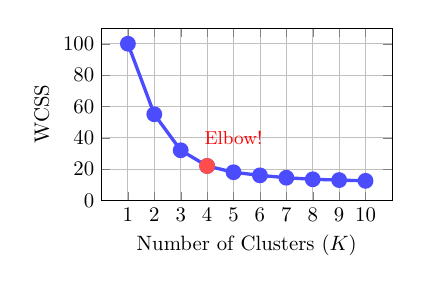
\begin{tikzpicture}[scale=0.75]
    \begin{axis}[
        width=6.5cm, height=4.5cm,
        xlabel={Number of Clusters ($K$)},
        ylabel={WCSS},
        grid=major,
        ymin=0, ymax=110,
        xmin=0, xmax=11,
        xtick={1,2,3,4,5,6,7,8,9,10},
        ytick={0,20,40,60,80,100}
    ]
    \addplot[blue!70, ultra thick, mark=*, mark size=3pt] coordinates {
        (1,100) (2,55) (3,32) (4,22) (5,18) (6,16) (7,14.5) (8,13.5) (9,13) (10,12.5)
    };
    \addplot[red!70, ultra thick, mark=*, mark size=3pt] coordinates {
        (4,22)
    };
    
    % Elbow annotation
    % \draw[red, very thick] (axis cs:2.5,20) -- (axis cs:4,20) -- (axis cs:4,35);
    \node[red, font=\small] at (axis cs:5,40) {Elbow!};
    % \draw[red, thick, ->] (axis cs:4.8,26) -- (axis cs:4,22);
    \end{axis}
\end{tikzpicture}

\vspace{0.3em}
\small Look for the "elbow" where adding more clusters doesn't help much (in the above case it is 4)
\end{column}

\end{columns}

\end{frame}

% --- SLIDE 7: Application 1 - Customer Segmentation ---
\begin{frame}{Application 1: Customer Segmentation}

\textbf{Use case:} Group customers for targeted marketing
\vspace{0.5em}

\begin{columns}[T] % align columns at the top

% ===================== LEFT COLUMN (Data & Plot) =====================
\begin{column}{0.48\textwidth}

    % Example Box
    \begin{tcolorbox}[
      colback=blue!5, colframe=blue!50,
      title=\textbf{Example: E-commerce Data},
      boxsep=3pt, left=4pt, right=4pt, top=3pt, bottom=3pt
    ]
    \small
    \begin{itemize}\setlength\itemsep{0.2em}
        \item Features: frequency, spend, recency
        \item Run K-Means with $K=4$
        \item Interpret clusters
    \end{itemize}
    \end{tcolorbox}

    \vspace{0.5em}
    
    % Scatter Plot
    \centering
    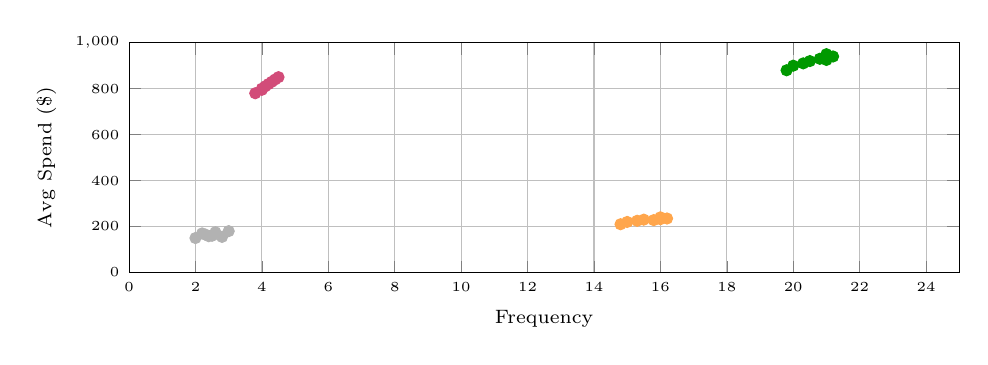
\begin{tikzpicture}
    \begin{axis}[
        width=\linewidth, height=4.5cm,
        xlabel={\scriptsize Frequency},
        ylabel={\scriptsize Avg Spend (\$)},
        grid=major,
        tick label style={font=\tiny},
        label style={font=\scriptsize},
        % legend style={font=\tiny, at={(0.02,0.98)}, anchor=north middle, fill opacity=0.8, draw=gray!20},
        xmin=0, xmax=25,
        ymin=0, ymax=1000
    ]
    % Inactive (Gray)
    \addplot[only marks, mark=*, mark size=2pt, gray!60] coordinates {
        (2,150) (3,180) (2.5,160) (2.2,170) (2.8,155)
        (2.3,165) (2.6,175) (2.4,158)
    };
    % Bargain (Orange)
    \addplot[only marks, mark=*, mark size=2pt, orange!70] coordinates {
        (15,220) (16,240) (15.5,230) (14.8,210) (16.2,235)
        (15.3,225) (15.8,228) (16,232)
    };
    % Big Spender (Purple)
    \addplot[only marks, mark=*, mark size=2pt, purple!70] coordinates {
        (4,800) (4.5,850) (4.2,820) (3.8,780) (4.3,830)
        (4.1,810) (4.4,840) (4.0,795)
    };
    % VIP (Green)
    \addplot[only marks, mark=*, mark size=2pt, green!60!black] coordinates {
        (20,900) (21,950) (20.5,920) (19.8,880) (21.2,940)
        (20.3,910) (20.8,930) (21,925)
    };
    % \legend{Inactive,Bargain,Big Spender,VIP}
    \end{axis}
    \end{tikzpicture}

\end{column}

% ===================== RIGHT COLUMN (Segments) =====================
\begin{column}{0.48\textwidth}
    \textbf{Discovered Segments:}
    \vspace{0.35em}

    % Inner Columns for the 2x2 grid
    \begin{columns}[T]
    
        % -- Inner Left --
        \begin{column}{0.48\textwidth}
            % Inactive Box
            \begin{tcolorbox}[colback=gray!10, colframe=gray!55,
              title=\centering\small\textbf{Inactive}, boxsep=2pt, left=2pt, right=2pt, top=2pt, bottom=2pt, height=2.4cm]
            \centering\small
            Low freq, \\low spend
            \vspace{0.3em}
            
            \textbf{Action:} \\Re-engage
            \end{tcolorbox}
            
            \vspace{0.3em}
            
            % Big Spender Box
            \begin{tcolorbox}[colback=purple!10, colframe=purple!55,
              title=\centering\small\textbf{Big Spenders}, boxsep=2pt, left=2pt, right=2pt, top=2pt, bottom=2pt, height=2.8cm]
            \centering\small
            Low freq, \\high spend
            \vspace{0.3em}
            
            \textbf{Action:} \\Premium Service
            \end{tcolorbox}
        \end{column}

        % -- Inner Right --
        \begin{column}{0.48\textwidth}
            % Bargain Box
            \begin{tcolorbox}[colback=orange!10, colframe=orange!55,
              title=\centering\small\textbf{Bargain}, boxsep=2pt, left=2pt, right=2pt, top=2pt, bottom=2pt, height=2.4cm]
            \centering\small
            High freq, \\low spend
            \vspace{0.3em}
            
            \textbf{Action:} \\Discounts
            \end{tcolorbox}
            
            \vspace{0.3em}
            
            % VIP Box
            \begin{tcolorbox}[colback=green!10, colframe=green!50!black,
              title=\centering\small\textbf{VIP}, boxsep=2pt, left=2pt, right=2pt, top=2pt, bottom=2pt, height=2.8cm]
            \centering\small
            High freq, \\high spend
            \vspace{0.3em}
            
            \textbf{Action:} \\Loyalty Program
            \end{tcolorbox}
        \end{column}
    \end{columns}
\end{column}

\end{columns}
\end{frame}
% --- SLIDE 8: Application 2 - Document Clustering (Simplified) ---
\begin{frame}{Application 2: Document Clustering}

\textbf{Use case:} Automatically organize news articles by topic.

% \vspace{1em}
\centering
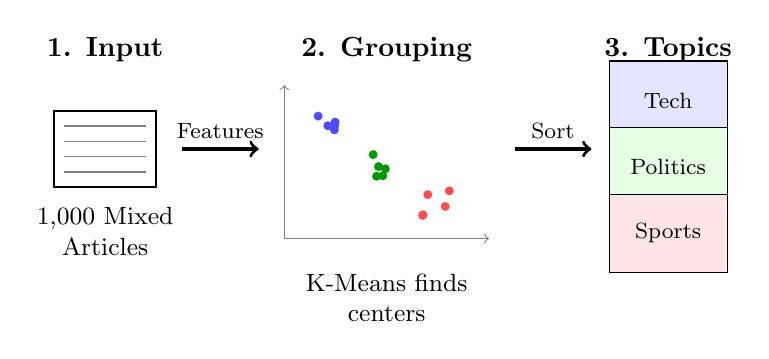
\begin{tikzpicture}[scale=0.65]
    % --- Step 1: Raw Documents (Left) ---
    \node[font=\bfseries] at (1, 4.2) {1. Input};
    
    % Simple document icons
    \draw[fill=white, thick] (0, 1.5) rectangle (2, 3);
    \foreach \y in {2.7, 2.4, 2.1, 1.8} {
        \draw[gray] (0.2, \y) -- (1.8, \y);
    }
    \node[below, align=center, font=\small] at (1, 1.3) {1,000 Mixed\\Articles};

    % Arrow 1
    \draw[->, very thick] (2.5, 2.25) -- (4, 2.25) node[midway, above, font=\footnotesize] {Features};

    % --- Step 2: Feature Space (Middle) ---
    \node[font=\bfseries] at (6.5, 4.2) {2. Grouping};
    
    % Axes
    \draw[->, gray] (4.5, 0.5) -- (8.5, 0.5);
    \draw[->, gray] (4.5, 0.5) -- (4.5, 3.5);

    % Clusters (simplified points)
    \foreach \i in {1,...,5} \fill[red!70] (7.5 + 0.3*rand, 1.2 + 0.3*rand) circle (2.5pt); % Sports
    \foreach \i in {1,...,5} \fill[blue!70] (5.2 + 0.3*rand, 2.8 + 0.3*rand) circle (2.5pt); % Tech
    \foreach \i in {1,...,5} \fill[green!60!black] (6.5 + 0.3*rand, 2.0 + 0.3*rand) circle (2.5pt); % Politics
    
    \node[below, align=center, font=\small] at (6.5, 0) {K-Means finds\\centers};

    % Arrow 2
    \draw[->, very thick] (9, 2.25) -- (10.5, 2.25) node[midway, above, font=\footnotesize] {Sort};

    % --- Step 3: Topics (Right) ---
    \node[font=\bfseries] at (12, 4.2) {3. Topics};

    % Folder Icons
    \node[draw, fill=blue!10, minimum width=1.5cm, minimum height=1cm, align=center, font=\footnotesize] at (12, 3.2) {Tech};
    \node[draw, fill=green!10, minimum width=1.5cm, minimum height=1cm, align=center, font=\footnotesize] at (12, 1.9) {Politics};
    \node[draw, fill=red!10, minimum width=1.5cm, minimum height=1cm, align=center, font=\footnotesize] at (12, 0.6) {Sports};

\end{tikzpicture}

% \vspace{1em}
\begin{tcolorbox}[colback=yellow!5, colframe=orange!40, title=\textbf{Process}]
\begin{itemize}
    \item Convert text into numbers (Text Features).
    \item Similar stories appear close together in space.
    \item K-Means automatically groups them into topics.
\end{itemize}
\end{tcolorbox}

\centering
\small \textit{Example: Google News grouping stories from different sources.}

\end{frame}

% --- SLIDE 9: Limitations of K-Means ---
\begin{frame}{When K-Means Fails}

\textbf{K-Means assumes spherical, equal-sized clusters}

\vspace{0.5em}
\begin{columns}[t]
\begin{column}{0.48\textwidth}
\textbf{Problem 1: Non-spherical}

\vspace{0.3em}
\centering
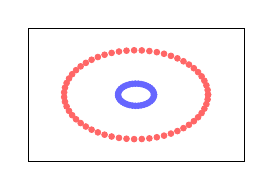
\begin{tikzpicture}[scale=0.7]
    \begin{axis}[
        width=5.5cm, height=4cm,
        grid=major,
        xmin=-3, xmax=3,
        ymin=-3, ymax=3,
        xtick=\empty, ytick=\empty
    ]
    
    % Two concentric circles
    \addplot[only marks, mark=*, mark size=1.5pt, blue!60, samples=40, domain=0:360] 
        ({0.5*cos(x)}, {0.5*sin(x)});
    \addplot[only marks, mark=*, mark size=1.5pt, red!60, samples=60, domain=0:360] 
        ({2*cos(x)}, {2*sin(x)});
    
    \end{axis}
\end{tikzpicture}

\vspace{0.2em}
\small {\color{red} Fails on concentric circles!}
\end{column}

\begin{column}{0.48\textwidth}
\textbf{Problem 2: Different sizes}

\vspace{0.3em}
\centering
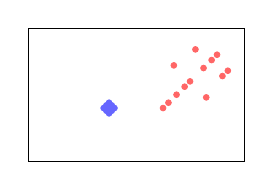
\begin{tikzpicture}[scale=0.7]
    \begin{axis}[
        width=5.5cm, height=4cm,
        grid=major,
        xmin=-3, xmax=5,
        ymin=-2, ymax=3,
        xtick=\empty, ytick=\empty
    ]
    
    % Small tight cluster
    \addplot[only marks, mark=*, mark size=1.5pt, blue!60] coordinates {
        (0,0) (0.1,0.1) (-0.1,0.1) (0.1,-0.1) (-0.1,-0.1)
        (0.2,0) (0,0.2) (-0.2,0) (0,-0.2)
    };
    
    % Large spread cluster
    \addplot[only marks, mark=*, mark size=1.5pt, red!60] coordinates {
        (3,1) (3.5,1.5) (2.5,0.5) (4,2) (2,0)
        (3.8,1.8) (2.2,0.2) (4.2,1.2) (2.8,0.8)
        (3.2,2.2) (3.6,0.4) (2.4,1.6) (4.4,1.4)
    };
    
    \end{axis}
\end{tikzpicture}

\vspace{0.2em}
\small {\color{red} Struggles with size differences!}
\end{column}
\end{columns}

\vspace{0.5em}
\begin{tcolorbox}[colback=yellow!8, colframe=orange!60, title=\textbf{Other Limitations}]
\begin{itemize}
\item Sensitive to outliers
\item Must specify $K$ in advance
\item Random initialization matters
\item Bad results for high dimensional data
\end{itemize}
\end{tcolorbox}

\vspace{0.3em}
\textbf{Alternatives:} DBSCAN (density-based), Gaussian Mixture Models, Hierarchical clustering

\end{frame}
% =========================
% PCA (Principal Component Analysis) - IMPROVED VERSION
% =========================

\section{Dimensionality Reduction: PCA}

% --- SLIDE 1: The Curse of Dimensionality ---
